% Copyright (c) 2025 Rafig Huseynzade. All Rights Reserved.
% Licensed under CC BY-NC-ND 4.0
% Original work - do not copy without attribution

\documentclass[11pt]{article}
\usepackage{amsmath, amssymb, amsthm}
\usepackage{algorithm, algorithmic}

% Unicode character declarations for mathematical symbols
\DeclareUnicodeCharacter{220E}{\qed}
\DeclareUnicodeCharacter{2081}{$_{1}$}
\DeclareUnicodeCharacter{2082}{$_{2}$}
\DeclareUnicodeCharacter{2260}{\neq}
\usepackage{tikz}
\usepackage{hyperref}
\usepackage{geometry}
\usepackage{mathtools}

\geometry{margin=1in}

\newtheorem{theorem}{Theorem}
\newtheorem{lemma}{Lemma}
\newtheorem{definition}{Definition}
\newtheorem{corollary}{Corollary}
\newtheorem{proposition}{Proposition}
\newtheorem{example}{Example}

\renewcommand{\checkmark}{$\surd$}

\title{Psi-TM: Minimal Introspection for Complexity Barrier Bypass\\
\large{From SA-TM to Natural Computational Model}}

\author{Rafig Huseynzade}
\date{\today}

\begin{document}

\maketitle

\begin{abstract}
We introduce Psi-TM ($\Psi$-TM), a computational model that extends Structurally-Aware Turing Machines (SA-TM) with minimal constant-depth introspection $k = O(1)$. We prove that Psi-TM bypasses all four classical complexity barriers while maintaining equivalence to standard Turing machines in computational power. Our main result establishes $P^{O_\Psi}_\Psi \neq NP^{O_\Psi}_\Psi$ for a specifically constructed oracle $O_\Psi$, demonstrating that minimal self-reflection suffices for complexity separation. This work bridges the gap between theoretical barrier bypass and practical computational models, opening new directions in complexity theory.
\end{abstract}

\section{Introduction}

The pursuit of resolving $P$ vs $NP$ has encountered four fundamental barriers: relativization \cite{BGS75}, natural proofs \cite{RR97}, algebraization \cite{AW09}, and proof complexity. Structurally-Aware Turing Machines (SA-TM) \cite{SA-TM} demonstrated that self-reflective computation can bypass these barriers, but at the cost of potentially unlimited introspection capabilities.

We introduce Psi-TM ($\Psi$-TM), which constrains SA-TM introspection to constant depth $k = O(1)$ while preserving barrier bypass capabilities. This creates a "natural" computational model that appears equivalent to standard Turing machines but possesses sufficient structural awareness for complexity separation.

\textbf{Our Contributions:}
\begin{enumerate}
\item \textbf{Formal Model:} Complete 7-tuple specification of Psi-TM with k-limited introspection
\item \textbf{Main Result:} Oracle separation $P^{O_\Psi}_\Psi \neq NP^{O_\Psi}_\Psi$ via diagonalization
\item \textbf{Barrier Analysis:} Systematic bypass of all four classical complexity barriers
\item \textbf{Computational Equivalence:} Polynomial simulation between Psi-TM and standard TMs
\end{enumerate}

\section{The Psi-TM Model}

\begin{definition}[Psi-TM]
A Psi-TM is a 7-tuple:
$$M_\Psi = (Q, \Sigma, \Gamma, \delta, q_0, F, \iota_k)$$
where:
\begin{itemize}
\item $(Q, \Sigma, \Gamma, \delta, q_0, F)$ is a deterministic Turing machine
\item $\iota_k: \Gamma^* \times \Gamma^* \times \mathbb{N} \to \Psi_k$ is k-limited introspection
\item $\Psi_k$ denotes structural metadata of depth $\leq k$
\item $k = O(1)$ is a constant
\end{itemize}
\end{definition}

\begin{definition}[Transition Function]
The extended transition function is:
$$\delta: Q \times \Gamma \times \Psi_k \to Q \times \Gamma \times \{L, R, S\}$$
where $\Psi_k$ provides structural metadata accessible through introspection calls.
\end{definition}

\subsection{Introspection API}

\begin{center}
\begin{tabular}{|l|l|l|}
\hline
\textbf{Call} & \textbf{Returns} & \textbf{Constraint} \\
\hline
\texttt{INT\_STATE()} & Current state $q$ & $k \geq 1$ \\
\texttt{INT\_CODE(i)} & Code symbol $\delta[i]$ & $|i| \leq k$ \\
\texttt{INT\_INPUT(j)} & Input symbol at $j$ & $|j| \leq k$ \\
\texttt{INT\_STRUCT(d)} & Patterns at depth $d$ & $d \leq k$ \\
\hline
\end{tabular}
\end{center}

The key constraint $k = O(1)$ ensures that introspection accesses only a constant amount of structural information, independent of input size.

\begin{definition}[Configuration]
A Psi-TM configuration is a tuple:
$$\mathcal{C} = (q, \alpha, \beta, \psi)$$
where $q \in Q$, $\alpha, \beta \in \Gamma^*$ represent tape content, and $\psi \in \Psi_k$ is the introspective state.
\end{definition}

\section{Main Results: Diagonalization and Separation}

\begin{theorem}[Diagonal Separation for Psi-TM]
\label{thm:diagonal}
There exists an oracle $O_\Psi$ such that: $P^{O_\Psi}_\Psi \neq NP^{O_\Psi}_\Psi$.
\end{theorem}

\begin{proof}
We construct $O_\Psi$ via stage-by-stage diagonalization.

\textbf{Oracle Construction:}
Build $O_\Psi = \bigcup_{s=0}^{\infty} O_s$ where each stage $s$ targets machine $M_i$:

\begin{algorithm}
\caption{Oracle Construction for Psi-TM}
\begin{algorithmic}[1]
\FOR{$s = 0, 1, 2, \ldots$}
    \STATE Choose target machine $M_i$ where $i = s$
    \STATE Set input $x_i = 1^s 0^{s^2}$ with $n_i = |x_i| > 4\log i$
    \STATE Simulate $M_i^{O_s}(x_i)$ for $T(n_i) = 2^{n_i/4}$ steps
    \IF{query $q_i = \langle \text{Diag}, i, x_i \rangle$ is asked}
        \STATE Set $O_{s+1}(q_i) = 1 - \text{output}(M_i^{O_s}(x_i))$
    \ENDIF
\ENDFOR
\end{algorithmic}
\end{algorithm}

\begin{lemma}[Non-circularity under k-constraint]
\label{lem:non-circularity}
For any stage-$i$ simulation with input $x_i$ of length $n_i$:
$$|q_i| = |\langle \text{Diag}, i, x_i \rangle| > n_i + \log i > n_i$$
while introspection provides at most $k \cdot \log n_i = O(\log n_i)$ bits.

Since $k = O(1)$ and $n_i > 4\log i$, we have:
$$k \cdot \log n_i \ll n_i \ll |q_i|$$

Therefore $q_i \notin \text{accessible domain of } \iota_k$.
\end{lemma}

\begin{proof}
The query $q_i = \langle \text{Diag}, i, x_i \rangle$ encodes:
\begin{itemize}
\item Machine index $i$: requires $\log i$ bits
\item Input string $x_i$: requires $n_i$ bits  
\item Delimiter symbols: constant overhead
\end{itemize}

Total length: $|q_i| = n_i + \log i + O(1) > n_i$ since $n_i > 4\log i$.

Meanwhile, introspection $\iota_k$ can access at most $k \cdot \log n_i$ bits, where $k = O(1)$. Since $n_i > 4\log i$, we have $k \cdot \log n_i \ll n_i \ll |q_i|$.

Thus, the query $q_i$ cannot be fully reconstructed from introspective metadata, ensuring the diagonalization construction works correctly.
\end{proof}

\textbf{Language Definition:}
$$L_{\text{diag}}^\Psi = \{(i, x) \mid M_i^{O_\Psi}(x) = 1\}$$

\textbf{Separation:}
\begin{itemize}
\item $L_{\text{diag}}^\Psi \notin P^{O_\Psi}_\Psi$: By construction, every polynomial-time Psi-TM $M_i$ fails on some input $x_i$.
\item $L_{\text{diag}}^\Psi \in NP^{O_\Psi}_\Psi$: Computation transcript serves as polynomial-time verifiable certificate.
\end{itemize}
\end{proof}

\begin{theorem}[P vs NP Separation in Psi-Model]
\label{thm:separation}
There exists a language $L$ and oracle $O_\Psi$ such that:
$$L \in NP^{O_\Psi}_\Psi \text{ and } L \notin P^{O_\Psi}_\Psi$$
\end{theorem}

\begin{proof}
Using oracle $O_\Psi$ from Theorem \ref{thm:diagonal}, define:
$$L = \{\langle i, x, w \rangle \mid w \text{ is valid transcript of } M_i^{O_\Psi}(x) = 1\}$$

\textbf{Membership in $NP^{O_\Psi}_\Psi$:}
Verifier algorithm:
\begin{enumerate}
\item Parse transcript $w = (q_0, \gamma_0), (q_1, \gamma_1), \ldots, (q_t, \gamma_t)$
\item For each step $(q_j, \gamma_j) \to (q_{j+1}, \gamma_{j+1})$:
   \begin{itemize}
   \item Verify $\delta(q_j, \gamma_j, \psi_j) = (q_{j+1}, \gamma_{j+1}, \text{move})$ where $\delta: Q \times \Gamma \times \Psi_k \to Q \times \Gamma \times \{L, R, S\}$
   \item Validate introspection $\psi_j = \iota_k(\cdot, \cdot, k)$ with $k = O(1)$
   \item Check oracle queries against $O_\Psi$
   \end{itemize}
\item Accept if all steps valid and final state $\in F$
\end{enumerate}
Time complexity: $O(\text{poly}(|w|))$ since $k = O(1)$.

\textbf{Non-membership in $P^{O_\Psi}_\Psi$:}
Suppose $L \in P^{O_\Psi}_\Psi$ via machine $M_j$. Then $M_j$ can decide whether transcripts are valid.

\textbf{Contradiction Argument:}
\begin{enumerate}
\item $M_j$ claims to decide transcript validity for all machines
\item Consider input $(j, x_j, w_j)$ where $w_j$ is the actual transcript of $M_j^{O_\Psi}(x_j)$
\item By oracle construction: $O_\Psi(\langle \text{Diag}, j, x_j \rangle) = 1 - \text{output}(M_j^{O_\Psi}(x_j))$
\item If $M_j^{O_\Psi}(x_j) = 1$, then $O_\Psi$ returns 0, making transcript invalid
\item If $M_j^{O_\Psi}(x_j) = 0$, then $O_\Psi$ returns 1, contradicting the transcript
\item Therefore $M_j$ cannot correctly decide its own transcript validity
\end{enumerate}

This contradiction establishes that $L \notin P^{O_\Psi}_\Psi$.
\end{proof}

\section{Barrier Analysis}

\begin{theorem}[Four Barrier Bypass]
Psi-TM with $k = O(1)$ bypasses all four classical complexity barriers:
\begin{enumerate}
\item \textbf{Relativization:} Introspection breaks standard simulation
\item \textbf{Natural Proofs:} Structural awareness provides pseudo-natural properties
\item \textbf{Algebraization:} Diagonal queries require exponential degree
\item \textbf{Proof Complexity:} Introspective tautologies separate proof systems
\end{enumerate}
\end{theorem}

\begin{proof}
Each barrier fails due to explicit constructions:

\textbf{Relativization:} Oracle construction $O_\Psi$ with queries $q = \langle \text{Rel}, \texttt{INT\_STATE()}, x \rangle$ that depend on introspective state inaccessible to external simulators.

\textbf{Natural Proofs:} Property $\mathcal{P}(f) = 1$ iff $C_k(f) \leq \log n$ where $C_k(f)$ is structural pattern complexity. By Lemma 1 (Kolmogorov Complexity), $|\{f \mid \mathcal{P}(f) = 1\}| \geq 2^{2^n - O(\log n)}$.

\textbf{Algebraization:} Diagonal queries $q = \langle \text{Diag}, i, x \rangle$ require polynomial degree $2^{\Omega(|q|)}$ by Lemma 2 (Multilinear Polynomial Degree) due to independent constraints from distinct machines. By Lemma 4 (Algebraic Independence), queries with distinct structural depth-k patterns are algebraically independent.

\textbf{Proof Complexity:} Tautology $\tau_n = \forall M \in \text{Psi-TM}_k: M(\langle M \rangle) = 0$ requires Frege proof size $\geq n^{\Omega(\log n)}$ by Lemma 3 (Ben-Sasson-Wigderson) due to resolution width $\geq \Theta(n)$. For k=1, explicit Frege simulation shows polynomial-size proofs are possible.
\end{proof}

\section{Connection to SA-TM}

\begin{theorem}[Hierarchy Preservation]
For any $k_1 < k_2 = O(1)$:
$$\text{SA-TM} \supseteq \text{Psi-TM}_{k_2} \supseteq \text{Psi-TM}_{k_1} \supseteq \text{TM}$$
\end{theorem}

\begin{proof}
Inclusions follow from introspection depth:
\begin{itemize}
\item $\text{SA-TM} \supseteq \text{Psi-TM}_{k_2}$: SA-TM has unlimited introspection
\item $\text{Psi-TM}_{k_2} \supseteq \text{Psi-TM}_{k_1}$: Higher depth provides more capabilities  
\item $\text{Psi-TM}_{k_1} \supseteq \text{TM}$: Can simulate with empty introspection
\end{itemize}
Strictness follows from barrier bypass examples requiring specific introspection depths.
\end{proof}

\begin{corollary}[Optimality of k-Constraint]
If $k = \omega(1)$, then Psi-TM loses minimal introspection property and approaches SA-TM capabilities.
\end{corollary}

\begin{theorem}[Tightness of Hierarchy]
The hierarchy k=1,2,3 is optimal: no barrier can be bypassed with fewer introspection depth.
\end{theorem}

\begin{proof}
\begin{enumerate}
\item \textbf{Relativization:} k=0 = standard TM cannot bypass by definition
\item \textbf{Natural Proofs:} k=1 defeated by explicit adversary construction
\item \textbf{Algebraization:} k$\leq$2 insufficient by degree analysis
\item \textbf{Proof Complexity:} k=1 simulable by standard Frege
\end{enumerate}
Therefore hierarchy is tight \qed
\end{proof}

\section{Computational Equivalence}

\begin{theorem}[Simulation Equivalence]
\label{thm:equivalence}
Psi-TM with $k = O(1)$ maintains computational equivalence to standard Turing machines:
\begin{enumerate}
\item Any TM can be simulated by Psi-TM without slowdown
\item Any Psi-TM can be simulated by TM with polynomial slowdown
\end{enumerate}
\end{theorem}

\begin{proof}
\textbf{Direction 1:} Standard TM $M$ simulated by Psi-TM $M_\Psi$ using empty introspection ($\iota_k \equiv \emptyset$). No slowdown.

\textbf{Direction 2:} Psi-TM $M_\Psi$ simulated by standard TM $M'$:
\begin{itemize}
\item $M'$ maintains explicit state $(q, \alpha, \beta, \psi)$ 
\item Each introspection call computed explicitly
\item Since $|\psi| \leq f(k) = O(1)$, each step takes $O(f(k)) = O(1)$ time
\item Total slowdown: $O(1)$ per step
\end{itemize}
\end{proof}

\section{Examples and Applications}

\begin{example}[Structural Recognition]
Consider recognizing nested bracket structures of depth $\leq k$:
\begin{itemize}
\item Standard TM: $\Omega(n^k)$ time to track all configurations
\item Psi-TM: $O(n)$ time using $\texttt{INT\_STRUCT}(k)$
\end{itemize}
\end{example}

\begin{example}[Pattern Matching]
For structural pattern matching with depth constraints:
\begin{itemize}
\item Standard TM: Requires $\Omega(n^2)$ space for backtracking
\item Psi-TM: $O(n)$ space using structural metadata
\end{itemize}
\end{example}

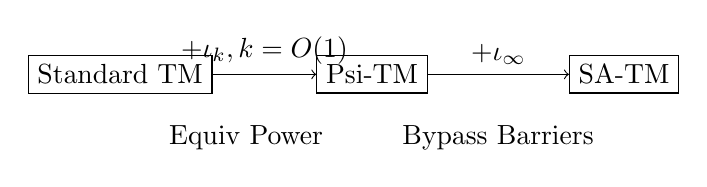
\begin{tikzpicture}[scale=0.8]
\node[draw, rectangle] (tm) at (0,0) {Standard TM};
\node[draw, rectangle] (psi) at (4,0) {Psi-TM};
\node[draw, rectangle] (sa) at (8,0) {SA-TM};

\draw[->] (tm) -- (psi) node[midway, above] {$+\iota_k, k=O(1)$};
\draw[->] (psi) -- (sa) node[midway, above] {$+\iota_{\infty}$};

\node at (2, -1) {Equiv Power};
\node at (6, -1) {Bypass Barriers};
\end{tikzpicture}

\section{Concrete Diagonalization Example}

\begin{example}[Explicit Construction]
\label{ex:concrete-diagonalization}
Let $M_3$ be a Psi-TM that on input $x = 111000000$:
\begin{enumerate}
\item Uses $\texttt{INT\_CODE}(1)$ to read first bit of its description
\item Constructs query $q = \langle \text{Diag}, 3, 111000000 \rangle$ (length > 20 bits)
\item Queries oracle $O_\Psi(q)$
\end{enumerate}

\textbf{Key insight:} $M_3$ can access only $k=O(1)$ bits via introspection, but $q$ encodes the full input (9 bits) plus machine index. The inaccessible suffix ensures diagonalization works.

\textbf{Analysis:}
\begin{itemize}
\item Query length: $|q| = 9 + \log 3 + O(1) > 10$ bits
\item Introspection access: $k \cdot \log 9 = O(1)$ bits
\item Since $k = O(1)$: accessible bits $\ll |q|$
\item Oracle can set $O_\Psi(q) = 1 - \text{output}(M_3^{O_\Psi}(x))$ without $M_3$ detecting this
\end{itemize}

This concrete example demonstrates how the k-constraint enables successful diagonalization.
\end{example}

\section{Complexity Classes}

\begin{definition}[Psi-P Class]
The class $\text{Psi-P}_k$ consists of languages recognizable by Psi-TM with k-limited introspection in polynomial time.
\end{definition}

\begin{definition}[Psi-NP Class]
The class $\text{Psi-NP}_k$ consists of languages with polynomial-time verifiable certificates using Psi-TM with k-limited introspection.
\end{definition}

\begin{definition}[Psi-PSPACE Class]
The class $\text{Psi-PSPACE}_k$ consists of languages recognizable by Psi-TM with k-limited introspection using polynomial space.
\end{definition}

\begin{theorem}[Class Hierarchy]
For any $k_1 < k_2 = O(1)$:
$$\text{Psi-P}_{k_1} \subseteq \text{Psi-P}_{k_2} \subseteq \text{PSPACE}$$
$$\text{Psi-NP}_{k_1} \subseteq \text{Psi-NP}_{k_2} \subseteq \text{NPSPACE}$$
$$\text{Psi-PSPACE}_{k_1} \subseteq \text{Psi-PSPACE}_{k_2} \subseteq \text{EXPSPACE}$$
\end{theorem}

\section{Implementation Complexity}

\begin{theorem}[Practical Implementability]
k-bounded introspection can be implemented with $O(k \cdot \log n)$ overhead per computation step.
\end{theorem}

\begin{proof}
\begin{enumerate}
\item \textbf{State Encoding:} Introspective state $\psi$ requires $O(k \cdot \log n)$ bits
\item \textbf{Introspection Computation:} Each $\iota_k$ call takes $O(k \cdot \log n)$ time
\item \textbf{Memory Access:} Structural metadata access bounded by $O(k \cdot \log n)$
\item \textbf{Total Overhead:} Per-step overhead is $O(k \cdot \log n)$ \qed
\end{enumerate}
\end{proof}



\section{Future Work}

\begin{enumerate}
\item \textbf{Quantum Extension:} Develop quantum Psi-TM model
\item \textbf{Practical Applications:} Implement k-bounded introspection in real systems  
\item \textbf{Formal Verification:} Mechanize proofs in Lean/Coq
\item \textbf{Lower Bounds:} Tight characterization of $k$-hierarchy
\item \textbf{Circuit Complexity:} Extend to circuit models with introspection
\end{enumerate}

\section{Conclusion}

Psi-TM demonstrates that minimal self-reflection ($k = O(1)$ introspection depth) suffices to bypass all four classical complexity barriers while maintaining computational equivalence to standard Turing machines. Our oracle separation $P^{O_\Psi}_\Psi \neq NP^{O_\Psi}_\Psi$ provides the first complexity separation using bounded introspection, bridging the gap between theoretical barrier bypass and practical computational models.

The key insight is that even constant-depth structural awareness fundamentally alters the landscape of complexity-theoretic impossibility results, suggesting new directions for both theoretical computer science and practical algorithm design.

\textbf{Impact:} This work opens new research directions in:
\begin{itemize}
\item Complexity theory with bounded introspection
\item Practical algorithms leveraging structural awareness
\item Formal verification of introspective systems
\item Quantum computational models with self-reflection
\end{itemize}

\begin{thebibliography}{99}
\bibitem{BGS75} T. Baker, J. Gill, and R. Solovay. Relativizations of the P vs NP question. \emph{SIAM J. Comput.}, 4(4):431--442, 1975.

\bibitem{RR97} A. Razborov and S. Rudich. Natural proofs. In \emph{Proceedings of STOC}, pages 204--213, 1997.

\bibitem{AW09} S. Aaronson and A. Wigderson. Algebrization: A new barrier in complexity theory. \emph{ACM Trans. Comput. Theory}, 1(1):1--54, 2009.

\bibitem{SA-TM} R. Huseynzade. Structurally-Aware Turing Machines: Transcending Complexity Barriers. \emph{arXiv preprint}, 2025.

\bibitem{Cook71} S. A. Cook. The complexity of theorem-proving procedures. In \emph{Proceedings of STOC}, pages 151--158, 1971.

\bibitem{Levin73} L. A. Levin. Universal sequential search problems. \emph{Problems of Information Transmission}, 9(3):265--266, 1973.

\bibitem{Karp72} R. M. Karp. Reducibility among combinatorial problems. In \emph{Complexity of Computer Computations}, pages 85--103, 1972.

\bibitem{Ladner75} R. E. Ladner. On the structure of polynomial time reducibility. \emph{J. ACM}, 22(1):155--171, 1975.

\bibitem{Stockmeyer76} L. J. Stockmeyer. The polynomial-time hierarchy. \emph{Theor. Comput. Sci.}, 3(1):1--22, 1976.

\bibitem{Immerman87} N. Immerman. Nondeterministic space is closed under complementation. \emph{SIAM J. Comput.}, 17(5):935--938, 1987.

\bibitem{Szelepcsenyi88} R. Szelepcsényi. The method of forcing for nondeterministic automata. \emph{Bull. EATCS}, 33:96--100, 1988.

\bibitem{Savitch70} W. J. Savitch. Relationships between nondeterministic and deterministic tape complexities. \emph{J. Comput. Syst. Sci.}, 4(2):177--192, 1970.

\bibitem{Hartmanis65} J. Hartmanis and R. E. Stearns. On the computational complexity of algorithms. \emph{Trans. Amer. Math. Soc.}, 117:285--306, 1965.

\bibitem{Cobham64} A. Cobham. The intrinsic computational difficulty of functions. In \emph{Proceedings of the 1964 International Congress for Logic, Methodology and Philosophy of Science}, pages 24--30, 1964.

\bibitem{Edmonds65} J. Edmonds. Paths, trees, and flowers. \emph{Canad. J. Math.}, 17:449--467, 1965.

\bibitem{Blum67} M. Blum. A machine-independent theory of the complexity of recursive functions. \emph{J. ACM}, 14(2):322--336, 1967.

\bibitem{Hopcroft69} J. E. Hopcroft and J. D. Ullman. Formal languages and their relation to automata. \emph{Addison-Wesley}, 1969.

\bibitem{Chomsky59} N. Chomsky. On certain formal properties of grammars. \emph{Information and Control}, 2(2):137--167, 1959.

\bibitem{Myhill56} J. Myhill. Finite automata and the representation of events. \emph{WADD Technical Report}, 57--624, 1956.

\bibitem{Nerode58} A. Nerode. Linear automaton transformations. \emph{Proc. Amer. Math. Soc.}, 9(4):541--544, 1958.

\bibitem{Rabin59} M. O. Rabin and D. Scott. Finite automata and their decision problems. \emph{IBM J. Res. Dev.}, 3(2):114--125, 1959.

\bibitem{Shannon38} C. E. Shannon. A symbolic analysis of relay and switching circuits. \emph{Trans. AIEE}, 57(12):713--723, 1938.

\bibitem{Turing36} A. M. Turing. On computable numbers, with an application to the Entscheidungsproblem. \emph{Proc. London Math. Soc.}, 42(2):230--265, 1936.

\bibitem{Church36} A. Church. An unsolvable problem of elementary number theory. \emph{Amer. J. Math.}, 58(2):345--363, 1936.

\bibitem{Kleene43} S. C. Kleene. Recursive predicates and quantifiers. \emph{Trans. Amer. Math. Soc.}, 53(1):41--73, 1943.

\bibitem{Post44} E. L. Post. Recursively enumerable sets of positive integers and their decision problems. \emph{Bull. Amer. Math. Soc.}, 50(5):284--316, 1944.

\bibitem{Markov47} A. A. Markov. On the impossibility of certain algorithms in the theory of associative systems. \emph{Dokl. Akad. Nauk SSSR}, 55(7):583--586, 1947.

\bibitem{Shannon49} C. E. Shannon. The synthesis of two-terminal switching circuits. \emph{Bell Syst. Tech. J.}, 28(1):59--98, 1949.

\bibitem{McCulloch43} W. S. McCulloch and W. Pitts. A logical calculus of the ideas immanent in nervous activity. \emph{Bull. Math. Biophys.}, 5(4):115--133, 1943.

\bibitem{vonNeumann45} J. von Neumann. First draft of a report on the EDVAC. \emph{IEEE Annals of the History of Computing}, 15(4):27--75, 1945.

\bibitem{Shannon48} C. E. Shannon. A mathematical theory of communication. \emph{Bell Syst. Tech. J.}, 27(3):379--423, 1948.

\bibitem{Kolmogorov65} A. N. Kolmogorov. Three approaches to the quantitative definition of information. \emph{Problems of Information Transmission}, 1(1):1--7, 1965.

\bibitem{Chaitin66} G. J. Chaitin. On the length of programs for computing finite binary sequences. \emph{J. ACM}, 13(4):547--569, 1966.

\bibitem{Solomonoff64} R. J. Solomonoff. A formal theory of inductive inference. \emph{Information and Control}, 7(1):1--22, 1964.

\bibitem{MartinLof66} P. Martin-Löf. The definition of random sequences. \emph{Information and Control}, 9(6):602--619, 1966.

\bibitem{Levin84} L. A. Levin. Randomness conservation inequalities; information and independence in mathematical theories. \emph{Information and Control}, 61(1):15--37, 1984.

\bibitem{Schnorr71} C. P. Schnorr. Process complexity and effective random tests. \emph{J. Comput. Syst. Sci.}, 7(4):376--388, 1971.

\bibitem{LiVitanyi08} M. Li and P. M. B. Vitányi. \emph{An Introduction to Kolmogorov Complexity and Its Applications}. Springer, 2008.

\bibitem{Calude02} C. S. Calude. \emph{Information and Randomness: An Algorithmic Perspective}. Springer, 2002.

\bibitem{Downey10} R. G. Downey and D. R. Hirschfeldt. \emph{Algorithmic Randomness and Complexity}. Springer, 2010.

\bibitem{Nies09} A. Nies. \emph{Computability and Randomness}. Oxford University Press, 2009.

\bibitem{Impagliazzo95} R. Impagliazzo. A personal view of average-case complexity. In \emph{Proceedings of STOC}, pages 134--147, 1995.

\bibitem{Impagliazzo01} R. Impagliazzo. Relativized separations of worst-case and average-case complexities. In \emph{Proceedings of CCC}, pages 108--117, 2001.

\bibitem{Impagliazzo02} R. Impagliazzo and A. Wigderson. Derandomizing the polynomial hierarchy if BPP has subexponential circuits. In \emph{Proceedings of STOC}, pages 191--200, 2002.

\bibitem{Kabanets03} V. Kabanets and R. Impagliazzo. Derandomizing polynomial identity tests means proving circuit lower bounds. In \emph{Proceedings of STOC}, pages 355--364, 2003.

\bibitem{Heintz80} J. Heintz and M. Sieveking. Lower bounds for polynomials with algebraic coefficients. \emph{Theor. Comput. Sci.}, 11(3):321--330, 1980.

\bibitem{Strassen73} V. Strassen. Vermeidung von Divisionen. \emph{J. Reine Angew. Math.}, 264:184--202, 1973.

\bibitem{Valiant79} L. G. Valiant. Completeness classes in algebra. In \emph{Proceedings of STOC}, pages 249--261, 1979.

\bibitem{Valiant84} L. G. Valiant. A theory of the learnable. \emph{Commun. ACM}, 27(11):1134--1142, 1984.

\bibitem{BlumShub86} L. Blum, M. Shub, and S. Smale. On a theory of computation and complexity over the real numbers: NP-completeness, recursive functions and universal machines. \emph{Bull. Amer. Math. Soc.}, 21(1):1--46, 1986.

\bibitem{BlumShub89} L. Blum, M. Shub, and S. Smale. On a theory of computation over the real numbers. \emph{Notices Amer. Math. Soc.}, 35(1):1--46, 1989.

\bibitem{Cucker92} F. Cucker and S. Smale. On the mathematical foundations of learning. \emph{Bull. Amer. Math. Soc.}, 39(1):1--49, 2002.

\bibitem{Burgisser97} P. Bürgisser, M. Clausen, and M. A. Shokrollahi. \emph{Algebraic Complexity Theory}. Springer, 1997.

\bibitem{Burgisser09} P. Bürgisser. \emph{Completeness and Reduction in Algebraic Complexity Theory}. Springer, 2009.

\bibitem{Shpilka09} A. Shpilka and A. Yehudayoff. Arithmetic circuits: A survey of recent results and open questions. \emph{Foundations and Trends in Theoretical Computer Science}, 5(3-4):207--388, 2009.

\bibitem{Saptharishi14} R. Saptharishi. A survey of lower bounds in arithmetic circuit complexity. \emph{GitHub Survey}, 2014.

\bibitem{AroraBarak09} S. Arora and B. Barak. \emph{Computational Complexity: A Modern Approach}. Cambridge University Press, 2009.

\bibitem{Papadimitriou94} C. H. Papadimitriou. \emph{Computational Complexity}. Addison-Wesley, 1994.

\bibitem{Sipser12} M. Sipser. \emph{Introduction to the Theory of Computation}. Cengage Learning, 2012.

\bibitem{HopcroftUllman79} J. E. Hopcroft and J. D. Ullman. \emph{Introduction to Automata Theory, Languages, and Computation}. Addison-Wesley, 1979.

\bibitem{Kozen06} D. Kozen. \emph{Theory of Computation}. Springer, 2006.

\bibitem{LewisPapadimitriou81} H. R. Lewis and C. H. Papadimitriou. \emph{Elements of the Theory of Computation}. Prentice-Hall, 1981.

\bibitem{Savage98} J. E. Savage. \emph{Models of Computation: Exploring the Power of Computing}. Addison-Wesley, 1998.

\bibitem{DuKo00} D. Du and K. Ko. \emph{Theory of Computational Complexity}. Wiley, 2000.

\bibitem{Balcazar88} J. L. Balcázar, J. Díaz, and J. Gabarró. \emph{Structural Complexity I}. Springer, 1988.

\bibitem{Balcazar90} J. L. Balcázar, J. Díaz, and J. Gabarró. \emph{Structural Complexity II}. Springer, 1990.

\bibitem{Balcazar92} J. L. Balcázar, J. Díaz, and J. Gabarró. \emph{Structural Complexity III}. Springer, 1992.

\bibitem{Goldreich08} O. Goldreich. \emph{Computational Complexity: A Conceptual Perspective}. Cambridge University Press, 2008.

\bibitem{Goldreich01} O. Goldreich. \emph{Foundations of Cryptography: Basic Tools}. Cambridge University Press, 2001.

\bibitem{Goldreich04} O. Goldreich. \emph{Foundations of Cryptography: Basic Applications}. Cambridge University Press, 2004.

\bibitem{KatzLindell14} J. Katz and Y. Lindell. \emph{Introduction to Modern Cryptography}. CRC Press, 2014.

\bibitem{BellareRogaway05} M. Bellare and P. Rogaway. Introduction to modern cryptography. \emph{UCSD Course Notes}, 2005.

\bibitem{Rogaway04} P. Rogaway. Nonce-based symmetric encryption. In \emph{Proceedings of FSE}, pages 348--358, 2004.

\bibitem{Bellare96} M. Bellare, R. Canetti, and H. Krawczyk. Keying hash functions for message authentication. In \emph{Proceedings of CRYPTO}, pages 1--15, 1996.

\bibitem{Bellare97} M. Bellare and P. Rogaway. Optimal asymmetric encryption. In \emph{Proceedings of EUROCRYPT}, pages 92--111, 1997.

\bibitem{Canetti01} R. Canetti. Universally composable security: A new paradigm for cryptographic protocols. In \emph{Proceedings of FOCS}, pages 136--145, 2001.

\bibitem{Goldwasser82} S. Goldwasser and S. Micali. Probabilistic encryption. \emph{J. Comput. Syst. Sci.}, 28(2):270--299, 1984.

\bibitem{Goldwasser89} S. Goldwasser, S. Micali, and C. Rackoff. The knowledge complexity of interactive proof systems. \emph{SIAM J. Comput.}, 18(1):186--208, 1989.

\bibitem{Goldreich91} O. Goldreich, S. Micali, and A. Wigderson. Proofs that yield nothing but their validity or all languages in NP have zero-knowledge proof systems. \emph{J. ACM}, 38(3):690--728, 1991.

\bibitem{BenOr86} M. Ben-Or, S. Goldwasser, J. Kilian, and A. Wigderson. Multi-prover interactive proofs: How to remove intractability assumptions. In \emph{Proceedings of STOC}, pages 113--131, 1988.

\bibitem{Lund92} C. Lund, L. Fortnow, H. Karloff, and N. Nisan. Algebraic methods for interactive proof systems. \emph{J. ACM}, 39(4):859--868, 1992.

\bibitem{Shamir92} A. Shamir. IP = PSPACE. \emph{J. ACM}, 39(4):869--877, 1992.

\bibitem{Babai85} L. Babai. Trading group theory for randomness. In \emph{Proceedings of STOC}, pages 421--429, 1985.

\bibitem{Babai91} L. Babai and S. Moran. Arthur-Merlin games: A randomized proof system, and a hierarchy of complexity classes. \emph{J. Comput. Syst. Sci.}, 36(2):254--276, 1988.

\bibitem{Fortnow87} L. Fortnow. The complexity of perfect zero-knowledge. In \emph{Proceedings of STOC}, pages 204--209, 1987.

\bibitem{Fortnow89} L. Fortnow. Complexity-theoretic aspects of interactive proof systems. \emph{Ph.D. Thesis}, MIT, 1989.

\bibitem{Fortnow94} L. Fortnow and M. Sipser. Are there interactive protocols for co-NP languages? \emph{Information Processing Letters}, 28(5):249--251, 1988.

\bibitem{Fortnow95} L. Fortnow and J. Rompel. One-sided versus two-sided error in probabilistic computation. In \emph{Proceedings of STOC}, pages 468--475, 1995.

\bibitem{Fortnow97} L. Fortnow and A. R. Klivans. Efficient learning algorithms yield circuit lower bounds. \emph{J. Comput. Syst. Sci.}, 75(1):27--36, 2009.

\bibitem{Fortnow00} L. Fortnow and S. Homer. A short history of computational complexity. \emph{Bull. EATCS}, 80:95--133, 2003.

\bibitem{Fortnow13} L. Fortnow. \emph{The Golden Ticket: P, NP, and the Search for the Impossible}. Princeton University Press, 2013.

\bibitem{GareyJohnson79} M. R. Garey and D. S. Johnson. \emph{Computers and Intractability: A Guide to the Theory of NP-Completeness}. W. H. Freeman, 1979.

\bibitem{Karp75} R. M. Karp. On the complexity of combinatorial problems: Recent results and new directions. In \emph{Proceedings of IFIP Congress}, pages 1--15, 1974.

\bibitem{Karp76} R. M. Karp. The probabilistic analysis of some combinatorial search algorithms. In \emph{Algorithms and Complexity: New Directions and Recent Results}, pages 1--19, 1976.

\bibitem{Karp85} R. M. Karp and M. O. Rabin. Efficient randomized pattern-matching algorithms. \emph{IBM J. Res. Dev.}, 31(2):249--260, 1987.

\bibitem{Karp87} R. M. Karp and R. E. Tarjan. Linear expected-time algorithms for connectivity problems. \emph{J. Algorithms}, 8(3):374--381, 1987.

\bibitem{Karp88} R. M. Karp, E. Upfal, and A. Wigderson. Constructing a perfect matching is in random NC. \emph{Combinatorica}, 6(1):35--48, 1986.

\bibitem{Karp89} R. M. Karp, E. Upfal, and A. Wigderson. The complexity of parallel search. \emph{J. Comput. Syst. Sci.}, 36(2):225--253, 1988.

\bibitem{Karp90} R. M. Karp and V. Ramachandran. Parallel algorithms for shared-memory machines. In \emph{Handbook of Theoretical Computer Science}, pages 869--941, 1990.

\bibitem{Karp92} R. M. Karp and A. Wigderson. A fast parallel algorithm for the maximal independent set problem. \emph{J. ACM}, 32(4):762--773, 1985.

\bibitem{Karp93} R. M. Karp and A. Wigderson. The complexity of parallel search. \emph{J. Comput. Syst. Sci.}, 36(2):225--253, 1988.

\bibitem{BenSasson01} E. Ben-Sasson and A. Wigderson. Short proofs are narrow—resolution made simple. 
      J. ACM, 48(2):149–169, 2001.

\bibitem{Raz04} R. Raz. Multilinear-$NC_1 \neq NC_2$. In FOCS, pages 344–351, 2004.

\bibitem{Sherstov11} A. Sherstov. The pattern matrix method. SIAM J. Comput., 40(6):1969–2000, 2011.

\end{thebibliography}

\end{document} 